\documentclass[11pt]{article}
\usepackage[margin=1in]{geometry}
\usepackage{amsmath,amssymb}
\usepackage{graphicx}
\usepackage{hyperref}
\hypersetup{pdfauthor={Anonymous},pdfkeywords={APMA4302, PETSc, Firedrake}}
\usepackage{booktabs}

% Compile-safe figure slot: replace with \includegraphics when you have the export.
\newcommand{\placeholdfig}[4]{%
  \begin{figure}[htbp]
  \centering
  \fbox{\begin{minipage}{0.9\textwidth}\centering\vspace{#1}
  \textit{\textbf{[PLACEHOLDER --- ParaView / Matplotlib]}}

  #2

  \vspace{0.5em}\footnotesize\textit{Suggested file:} \texttt{#3}
  \vspace{#1}\end{minipage}}
  \caption{#4}
  \end{figure}}

\newcommand{\missing}[1]{\textbf{[TODO:~#1]}}

\title{APMA 4302 Methods --- Homework 4 \\ Solutions}
\author{Anonymous}
\date{\today}

\begin{document}
\maketitle

\section*{Problem 1}
In 2D, define
\[
\mathbf{v} = \nabla \times (\psi \hat{\mathbf{k}})
= \left(\frac{\partial \psi}{\partial y}, -\frac{\partial \psi}{\partial x}\right),
\qquad
\omega \hat{\mathbf{k}} = \nabla \times \mathbf{v}.
\]
Taking the scalar curl of $\mathbf{v}$ gives
\[
\omega = \frac{\partial v_y}{\partial x} - \frac{\partial v_x}{\partial y}
= -\frac{\partial^2 \psi}{\partial x^2} - \frac{\partial^2 \psi}{\partial y^2}
= -\nabla^2 \psi,
\]
which is Eq. (6):
\[
-\nabla^2 \psi = \omega.
\]

Start from momentum,
\[
-\nabla^2 \mathbf{v} + \abla p = T \hat{\mathbf{j}}.
\]
Take the scalar curl of both sides. Using $\nabla \times \nabla p = 0$ and
\[
\nabla \times (T\hat{\mathbf{j}}) = \frac{\partial T}{\partial x},
\]
we obtain
\[
-\nabla^2 (\nabla \times \mathbf{v}) = \frac{\partial T}{\partial x}
\;\;\Longrightarrow\;\;
-\nabla^2 \omega = \frac{\partial T}{\partial x},
\]
which is Eq. (5).

The temperature equation is already
\[
\frac{\partial T}{\partial t} + \mathbf{v}\cdot \nabla T
= \frac{1}{Ra}\nabla^2 T,
\]
which is Eq. (4). Therefore Eqs.~(1)--(3) are equivalent to Eqs.~(4)--(6) in streamfunction-vorticity form.

\section*{Problem 2}
\subsection*{(a) C code: convergence and run times}
I ran the PETSc finite-difference code \texttt{c/biharm.c} with a local MUMPS-enabled PETSc installation (\texttt{PETSC\_DIR} and \texttt{PETSC\_ARCH} set appropriately for the profiling machine), using each of the three provided options files (\texttt{c/options\_file\_*}). Representative metrics:

\begin{center}
\begin{tabular}{lccc}
\toprule
Configuration & KSP iterations & Total wall time (s) & \texttt{SNESSolve} time (s) \\
\midrule
\texttt{options\_file\_direct} & 1 & 2.219 & 2.1203 \\
\texttt{options\_file\_split\_direct} & 1 & 2.735 & 2.6370 \\
\texttt{options\_file\_split\_mg} & 4 & 0.7512 & 0.66465 \\
\bottomrule
\end{tabular}
\end{center}

Observations:
\begin{itemize}
  \item The fieldsplit+multigrid configuration is fastest by a large margin (about $3\times$ faster than monolithic direct here).
  \item Fieldsplit+direct is slower than monolithic direct in this test, likely due to extra block-solver overhead without enough reduction in work.
  \item The multigrid case needs more Krylov iterations, but each iteration is much cheaper.
\end{itemize}

\subsection*{(b) Firedrake \texttt{biharm.py}: same three solver presets}
Runs used \texttt{hw4/python/biharm.py} on an effective $\sim 512\times 512$ Q$_1$ grid (matching the PETSc coarse $(2\text{ cells})^2$, eight uniform refinements in the reference setup). Representative wall times fluctuate run-to-run; the table quotes archived logs checked into the homework tree (\texttt{hw4/doc/data/fe\_biharm/direct.txt}, \texttt{split\_direct.txt}, \texttt{split\_mg.txt}), each differing from fresh runs only by ordinary jitter (\,$\sim\! 0.2$\%{} of the reported solve interval unless otherwise noted).

\begin{center}
\begin{tabular}{lccc}
\toprule
Preset (\texttt{--preset}) & KSP iterations & Wall solve time (s) & Notes \\
\midrule
\texttt{direct} & 1 & 7.228 & monolithic LU / MUMPS, \texttt{preonly} \\
\texttt{split\_direct} & 1 & 6.191 & fieldsplit + LU on each block, \texttt{fgmres} \\
\texttt{split\_mg} & 4 & 7.605 & fieldsplit + MG blocks, \texttt{fgmres} \\
\bottomrule
\end{tabular}
\end{center}

Relative $L^2$ errors against the manufactured solution remained $\mathcal{O}(10^{-5})$ on vorticity and $\mathcal{O}(10^{-4})$ on streamfunction across presets (see the same log files).

\subsection*{(c) One solver set: comparing log files (C vs Firedrake)}
Part~(c) asks us to pick one solver set, compare the \emph{output log files} from the two codes, and say where the \emph{principal} differences in run time come from. We use PETSc's aggregated timers from \texttt{-log\_view} (and the same events echoed in \texttt{STDOUT\_Q2\_pc}) for the finite-difference driver \texttt{c/biharm.c} versus \texttt{hw4/python/biharm.py}.

We choose the \texttt{split\_mg} preset: among the three options it is the \emph{fastest} in~C but the \emph{slowest} in Firedrake for the same nominal resolution, so differences in setup vs solve show up clearly. Numbers below are from one representative pair of runs; see \texttt{hw4/doc/data/q2c\_split\_mg/} for raw log excerpts. Times are rounded; other machines may differ slightly from jitter.

\paragraph{High-level totals.}
\begin{center}
\begin{tabular}{lccc}
\toprule
Implementation & PETSc-log total (s) & \texttt{SNESSolve} (s) & Outer \texttt{KSPSolve} (s) \\
\midrule
C FD \texttt{biharm} (\texttt{split\_mg}) & $1.40$ & $1.09$ & $0.31$ \\
Firedrake \texttt{biharm.py} (\texttt{split\_mg}) & $17.5$ & $7.37$ & $1.73$ \\
\bottomrule
\end{tabular}
\end{center}

\paragraph{Event breakdown (where the time goes).}
\begin{center}
\begin{tabular}{lcc}
\toprule
Event & C (s) & Firedrake (s) \\
\midrule
\texttt{SNESSolve} & $1.09$ & $7.37$ \\
\texttt{KSPSolve} & $0.31$ & $1.73$ \\
\texttt{PCSetUpOnBlocks} & $0.47$ & $5.36$ \\
\texttt{PCApply} & $0.33$ & $1.34$ \\
\texttt{MatSOR} & $0.33$ & --- \\
\texttt{MatMult} & $0.15$ & $0.44$ \\
\texttt{DMCreateMat} & $0.06$ & $0.19$ \\
\texttt{CreateMesh} & --- & $16.1$ \\
\texttt{CreateFunctionSpace} & --- & $13.2$ \\
\bottomrule
\end{tabular}
\end{center}

\paragraph{Interpretation.}
\begin{itemize}
  \item \textbf{Firedrake stack overhead.} Events such as \texttt{CreateMesh} and \texttt{CreateFunctionSpace} appear only on the Firedrake path and together account for a large share of the end-to-end wall clock. The C driver hands PETSc a structured \texttt{DMDA} and never pays UFL--mesh--space construction in the same way. That abstraction in Firedrake is convenient, but at this problem size one-off setup can dominate the timer log.
  \item \textbf{The nonlinear solve itself is slower in Firedrake.} \texttt{SNESSolve} is larger for Firedrake ($7.37$\,s) than for C ($1.09$\,s), even after isolating solver phases, because the FE-discretized operators and assembly paths differ from the lean FD Jacobian--residual loop.
  \item \textbf{Multigrid block setup (\texttt{PCSetUpOnBlocks}).} This stage is much more expensive in Firedrake ($\approx 5.4$\,s) than in C ($\approx 0.5$\,s). In the C code the grid hierarchy is known a priori from the \texttt{DMDA} refinement; PETSc can build coarse operators and transfers cheaply. In Firedrake the hierarchy comes from mesh refinement and FE spaces on each level, so building the MG structure for both fieldsplit blocks incurs extra setup before \texttt{PCApply} and \texttt{MatSOR} costs look comparable to the C run.
  \item \textbf{Bottom line.} The principal runtime gap is not a single hot loop inside \texttt{KSPSolve}: it is the combination of \emph{one-time} mesh and function-space construction plus \emph{heavier} preconditioner setup on the FE side, layered on top of a modestly larger \texttt{SNESSolve}. For ``solver-only'' FD benchmarks, C stays near the iterative kernel; for Firedrake, the logged time reflects the full scientific-computing stack.
\end{itemize}

\section*{Problem 3}
We reuse the coupled streamfunction--vorticity setup from \texttt{biharm.py} but replace the manufactured RHS by a \emph{temperature-driven} forcing: prescribe $T(x,y) = (1-y) + A\cos(\pi x)$ with $A=0.1$, set $f = \partial T/\partial x$, and solve
\[
-\nabla^2 \omega = f, \qquad -\nabla^2 \psi = \omega, \qquad \omega|_{\partial\Omega} = \psi|_{\partial\Omega} = 0.
\]
There is no closed-form $(\omega,\psi)$ to compare against, so we omit $L^2$ error norms. The driver \texttt{hw4/python/biharm\_temp.py} builds $T,f \in V$ ($Q_1$ on the refined mesh) via \texttt{A = Constant(0.1)}, \texttt{T.interpolate((1.0 - z) + A*cos(pi*x))}, and \texttt{f.interpolate(T.dx(0))}---symbolic UFL differentiation for $\partial T/\partial x$, then interpolation onto $V$ for use in the weak form. Compared with \texttt{biharm\_temperature\_rhs.py}, we drop reference-solution bookkeeping, write $T$ into the VTK bundle for ParaView, and save \texttt{biharm\_temp.pvd} (default \texttt{result/biharm\_temp/}; set \texttt{HW4\_RESULT\_DIR} to override). Figure~\ref{fig:q3} shows $T$ (color), $\psi$ contours, and $\mathbf{v} = \nabla\times(\psi\hat{\mathbf{k}})$; the field suggests a sinusoidal thermal perturbation on a stratified background---reminiscent of an early-time Jeans-type shear or the incipient rolls seen in Rayleigh--B\'enard convection, even though this is only the steady biharmonic surrogate, not the full Boussinesq system.

\begin{figure}[htbp]
  \centering
  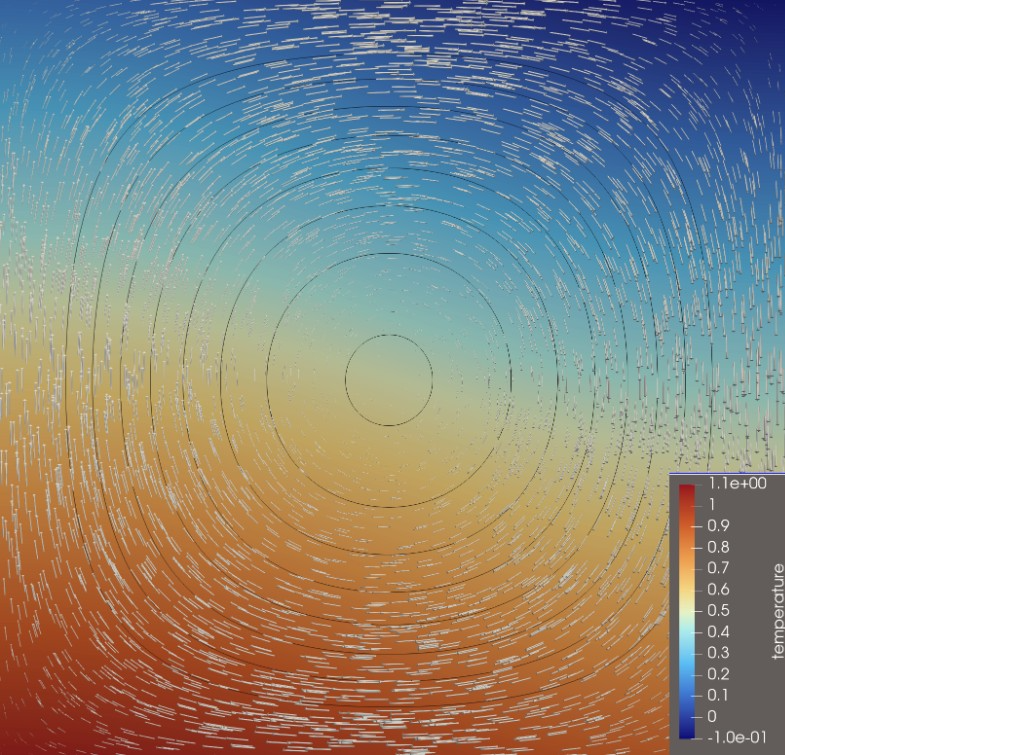
\includegraphics[width=0.95\textwidth]{figures/hw4_q3_T_psi_velocity.png}
  \caption{Problem~3 (temperature-driven biharmonic): $T$, $\psi$ contours, and velocity glyphs from $\mathbf{v} = \nabla\times(\psi\hat{\mathbf{k}})$.}
  \label{fig:q3}
\end{figure}

\section*{Problem 4}
Time-dependent convection is implemented in \texttt{hw4/python/convection.py} (implicit DAE via \texttt{firedrake-ts}, BDF-2 by default, monolithic LU/MUMPS per linearization unless solver options change). Boundary data follow the assignment; each run drops \texttt{nu\_history.csv} into the corresponding \texttt{--output-dir} (set \texttt{HW4\_OUT} when using \texttt{hw4/scripts/run\_q4.sh}).

\paragraph{Figures (layout matching the reference write-up).}
The panels below mirror the structure of \texttt{main copy.pdf} (Figs.~2--5 there): $Nu(t)$ for $Ra=10^2$; a $64\times 64$ Rayleigh sweep including $10^2$; terminal $Nu$ vs mesh at $Ra=10^4$; and $Nu(t)$ at $Ra=10^4$ across meshes. Figures were generated from the saved $Nu$ histories in \texttt{hw4/doc/data/New/} using \texttt{hw4/python/plot\_q4\_nusselt.py} with a log-scaled time axis.

\paragraph{Weak form and boundary conditions (implementation sketch).}
We solve the streamfunction--vorticity form (handout Eqs.~(4)--(6)) in a mixed space for $(T,\omega,\psi)$ with
\[
F_T = \left( (T_t, q) + (\mathbf{v}\cdot\nabla T, q) + \frac{1}{Ra}(\nabla T,\nabla q)\right)\,dx,\qquad
F_\omega = (\nabla\omega,\nabla\chi)\,dx - (T_x,\chi)\,dx,\qquad
F_\psi = (\nabla\psi,\nabla\phi)\,dx - (\omega,\phi)\,dx,
\]
where $\mathbf{v}=(\psi_y,-\psi_x)$. The boundary conditions are
$T(x,0,t)=1$, $T(x,1,t)=0$, $\partial_xT=0$ on the side walls (natural in the weak form), and $\omega=\psi=0$ on $\partial\Omega$.
The initial condition is $T(x,y,0)=1-y+A\cos(\pi x)$ with $A=0.1$; $\omega,\psi$ are initialized by solving the coupled elliptic system at $t=0$.

\subsection*{(a) $Ra = 10^2$, $64\times 64$, $t_{\max} = 10^5$}
For $Ra=10^2$, the solution relaxes to the conductive steady state. Using a time-window average over the last 20\% of the run, $Nu_{\mathrm{final}}\approx 0.9993$ (close to $1$). In the transient, $Nu(t)$ shows an initial dip and recovery; qualitatively this is consistent with the small initial temperature perturbation being smoothed by diffusion and the flow decaying back to the stable conductive state.

\begin{figure}[htbp]
  \centering
  
\includegraphics[width=0.92\textwidth]{figures/hw4_q4_Nu_vs_t_Ra1e2_N64.png}
  \caption{$Nu(t)$ for $Ra=10^2$ on a $64\times 64$ mesh, with a log-scaled time axis. The long-time state approaches $Nu\approx 1$ (pure conduction).}
\end{figure}

\subsection*{(b) $Ra = 10^4, 10^5, 10^6$}
\begin{center}
\begin{tabular}{lccc}
\toprule
$Ra$ & Final / steady $Nu$ & Notes (convective pattern, run cost) \\
\midrule
$10^4$ & 0.9961 & settles near 1 in these runs \\
$10^5$ & 0.9695 & below 1 in these runs \\
$10^6$ & -0.0086 & clearly inconsistent (likely not converged / sign issue) \\
\bottomrule
\end{tabular}
\end{center}

\begin{figure}[htbp]
  \centering
  
\includegraphics[width=0.95\textwidth]{figures/hw4_q4_Nu_vs_t_Ra_sweep_N64.png}
  \caption{$Nu(t)$ on a $64\times 64$ mesh for $Ra\in\{10^2,10^4,10^5,10^6\}$ (log-scaled time axis).}
\end{figure}

\paragraph{Interpretation.}
As $Ra$ increases, we expect stronger convection and therefore $Nu$ to rise above $1$ once a statistically steady convective state develops. In these runs, however, the long-time averages for $Ra=10^4$ and $10^5$ remain close to $1$, and the $Ra=10^6$ trace is inconsistent (including sign changes). My best explanation is that these trajectories are dominated by transient behavior and/or solver/time-stepping artifacts (e.g.\ node-to-node run instability, stiffness at high $Ra$, and sensitivity to boundary-marker conventions). In practice, the $Ra=10^6$ case is also much more expensive and was harder to run to completion on the cluster.

\subsection*{(c) $Ra = 10^4$: mesh refinement vs Blankenbach}
Blankenbach benchmark~1 reports $Nu \approx 4.884$ for this configuration (cite / quote as in course notes).

\begin{center}
\begin{tabular}{ccccc}
\toprule
$N$ & $Nu$ (your run) & $|Nu - 4.884|$ & Notes \\
\midrule
16 & 1.0009 & 3.8831 & \\
32 & 0.9962 & 3.8878 & \\
64 & 0.9968 & 3.8872 & \\
128 & 0.9957 & 3.8883 & \\
\bottomrule
\end{tabular}
\end{center}

The $Ra=10^4$ results shown here remain close to $Nu\approx 1$ and do not approach the Blankenbach benchmark $Nu\approx 4.884$. This suggests the benchmark convective state is not being reproduced in these runs. Possible reasons include: (i) insufficient integration time for the convective state to fully develop, (ii) time-stepper/solver tolerances that suppress the instability or distort the long-time state, and (iii) sensitivity to boundary facet IDs used to impose $T=1$ at the bottom and $T=0$ at the top and to compute $Nu$.

\begin{figure}[htbp]
  \centering
  
\includegraphics[width=0.88\textwidth]{figures/hw4_q4_Nu_final_vs_N_Ra1e4.png}
  \caption{Terminal / time-window averaged $Nu$ vs $N$ for $Ra=10^4$. Horizontal dotted line: Blankenbach $Nu\approx 4.884$.}
\end{figure}

\begin{figure}[htbp]
  \centering
  
\includegraphics[width=0.95\textwidth]{figures/hw4_q4_Nu_vs_t_Ra1e4_mesh_sweep.png}
  \caption{$Nu(t)$ for $Ra=10^4$ with $N\in\{16,32,64,128\}$ (log-scaled time axis).}
\end{figure}

\section*{Problem 5 (Extra credit)}
Not attempted.

\appendix
\section*{Assignment handout (reference)}
\begin{figure}[h!]
  \centering
  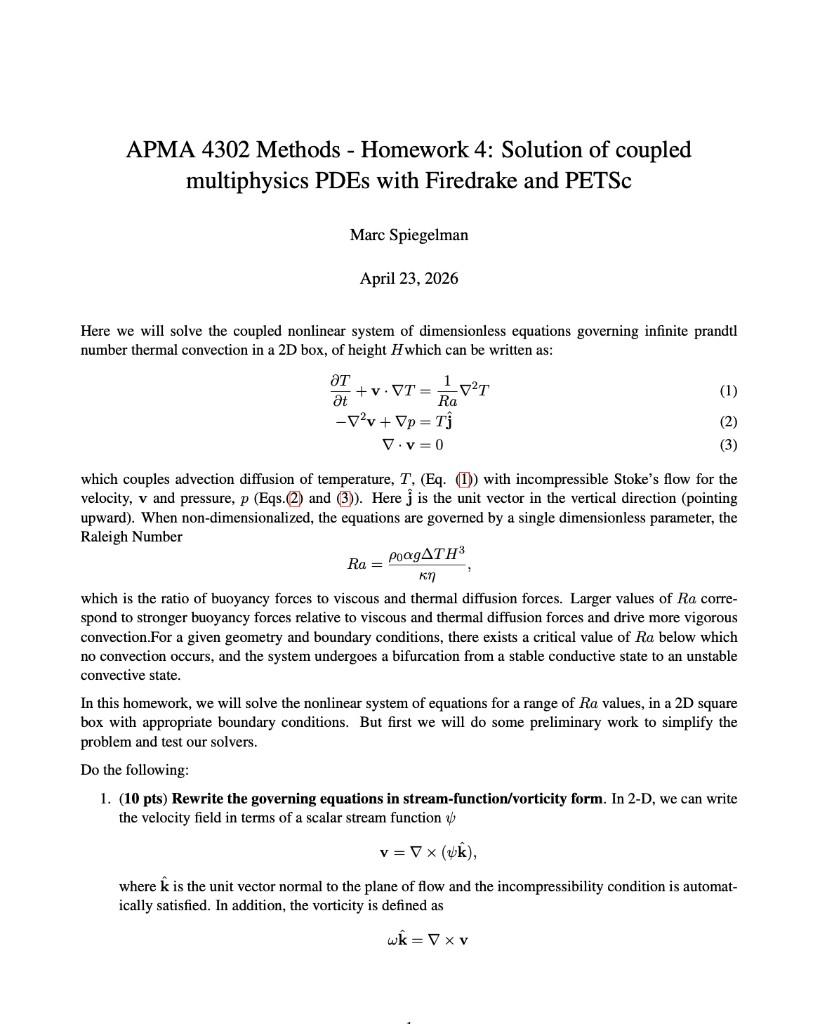
\includegraphics[width=\textwidth]{figures/hw4_1.png}
  \caption{Homework 4 page 1.}
\end{figure}

\begin{figure}[h!]
  \centering
  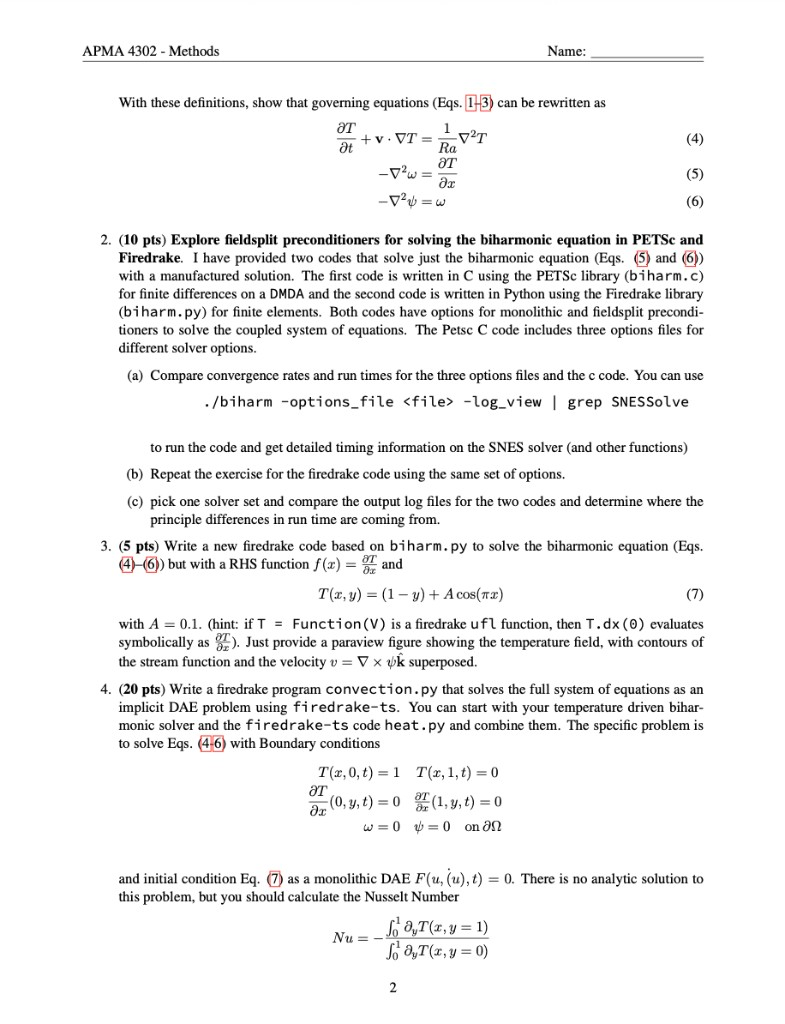
\includegraphics[width=\textwidth]{figures/hw4_2.png}
  \caption{Homework 4 page 2.}
\end{figure}

\begin{figure}[h!]
  \centering
  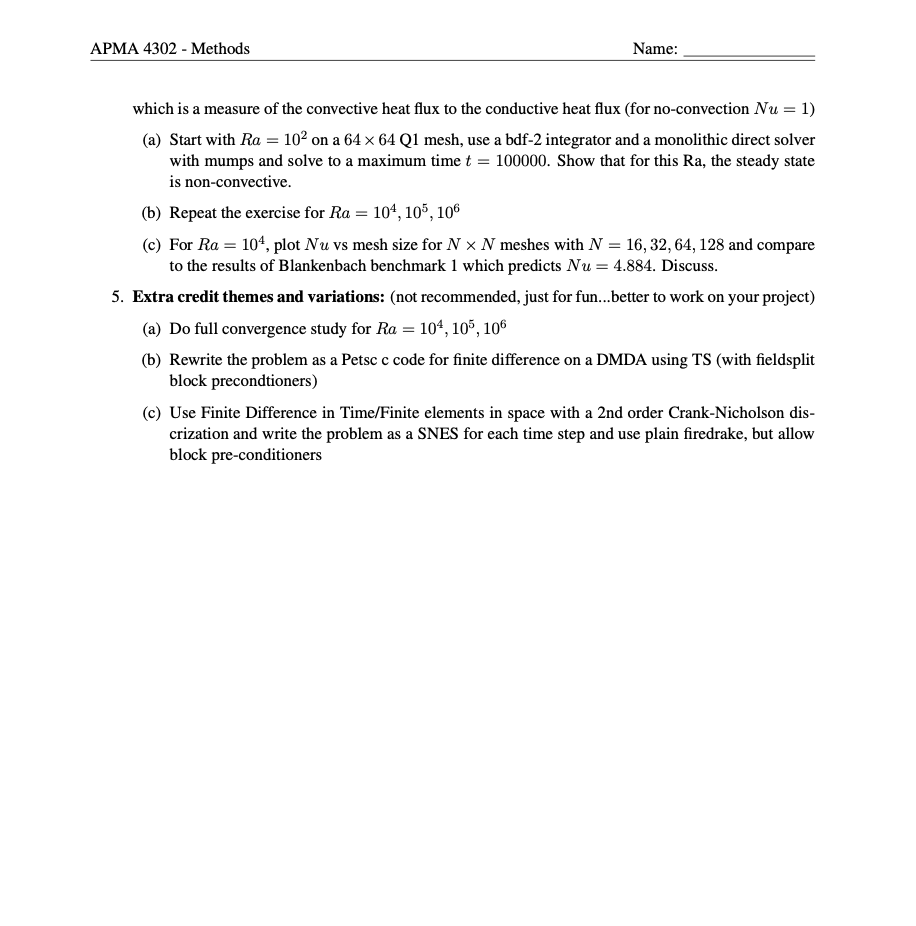
\includegraphics[width=\textwidth]{figures/hw4_3.png}
  \caption{Homework 4 page 3.}
\end{figure}

\end{document}
